\documentclass[12pt]{article}

\usepackage{amsmath}
\usepackage{color}
\definecolor{mygreen}{RGB}{28,172,0} % color values Red, Green, Blue
\definecolor{mylilas}{RGB}{170,55,241}
\usepackage{courier}
\usepackage{listings}
\usepackage{graphicx}
\usepackage[a4paper, total={6.5in, 8in}]{geometry}
\usepackage{float}
\usepackage[T1]{fontenc}
\usepackage{xcolor}
\usepackage{titlepic}
\usepackage{caption}
\captionsetup[figure]{labelfont=bf}
\usepackage{textcomp}
\usepackage[nottoc,numbib]{tocbibind}
\usepackage[justification=centering]{caption}
\usepackage{chronosys}

\def\chron@selectmonth#1{\ifcase#1\or Januar\or Februar\or März\or April\or Mai\or Juni\or Juli\or August\or September\or Oktober\or November\or Dezember\fi}

\setlength{\parindent}{0em}
\setlength{\parskip}{1em}
\renewcommand{\baselinestretch}{1.2}

\begin{document}

\pagenumbering{gobble}

\title{\textbf{Object Relational Anomaly Detection for Scene Analysis}\bigbreak
Master Thesis Proposal}
\author{Sashidhar Reddy Kanuboddi}

\maketitle

\titlepic{
\includegraphics[scale = 0.3]{university.jpeg}}

\newpage

\tableofcontents{}

\pagenumbering{arabic}

\newpage

\section{Motivation}

Autonomous mobile robots typically operate in dynamic environments that consist of multiple types of objects. These objects are usually scattered all over the environment. As humans, we have an expectation of which objects should be in the scene and where each object should ideally be located, based on our countless observations of similar environments beforehand.

The motivation of this thesis is to enable robots to have a similar understanding of its surroundings. The objective is to implement a learning framework that uses annotated 3D point clouds of different configurations of a particular type of scene, say a living room or an office, to extract features relevant to each object (such as its dimensions), the positional and angular bearings of each object with respect to other objects; learns from these features; and finally, is able to identify anomalous scenes when presented with new unseen instances of the scene based on what it has learnt from all the training instances.




\section{Modeling Spatial Relations of Objects in a Scene}

This thesis will essentially implement a framework from STRANDS, a collaborative European research project \cite{STRANDS}. The steps to implement the framework are as follows:

\begin{enumerate}
\item{Collecting a dataset of point clouds, consisting of different configurations of a particular type of scene.}
\item{Manually annotating each point cloud with 3D bounding boxes placed over each object.}
\item{Extracting features from this annotated point cloud dataset, such as pose and angular bearing of each object w.r.t a fixed frame of reference and w.r.t other objects, volume of each object etc.}
\item{Fitting a model over the extracted features, eg. a Gaussian Mixture Model.}
\item{Using the fitted model to compute scene similarity score for new scenes. Scenes with a score below a certain threshold would be declared anomalous.}
\end{enumerate}





\section{Thesis}

Each of the above mentioned steps is described in more detail below:

\subsection{Dataset of Point Clouds}

The idea, at the moment, is to capture the point cloud of a shelf filled with objects in order to learn about the underlying structure of which objects go where on the shelf. 

Let $S_t$ be a set of $n$ scenes $\{s_1, s_2,...., s_n\}$, where each scene is that of a shelf with a few objects. For example, in $s_1$, the shelf may contain just books, in $s_2$, the shelf may contain a small mug along with some books and so on. The scene is always that of the same shelf, but just like in the real world, although most of the times the shelf will have the same objects at the same locations, sometimes some additional objects may be present or sometimes, an object can be placed at a different location than its usual one.

Capturing the point clouds is not a trivial task, as we need high resolution point clouds of the entire scene, which means scanning with a 3D sensor (Microsoft Kinect, Asus Xtion) over multiple passes and fusing the point cloud from each pass to form one dense high resolution point cloud. A software called KinectFusion from Microsoft Research\cite{KinectFusion} claims to accomplish this task in real time with the help of heavy graphics hardware and it is proposed to use this tool in this thesis.


\begin{figure} [H]
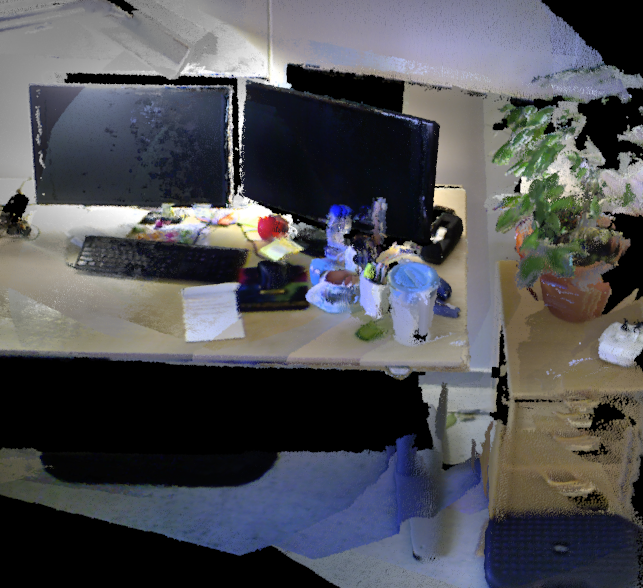
\includegraphics[scale = 0.25]{pcl.png}
\centering
\caption{\textbf{High Resolution Point Cloud of an Office Desk \cite{KTH Dataset}}} 
\end{figure}


\subsection{Manual Annotation of the Dataset}

Once the point clouds have been gathered, each of them will be manually annotated using a tool developed by the STRANDS project for their research. This tool allows us to graphically put 3D bounding boxes over each object in the scene and export information about the pose (w.r.t a fixed frame of reference) and dimensions of each bounding box to an XML file.

\begin{figure} [H]
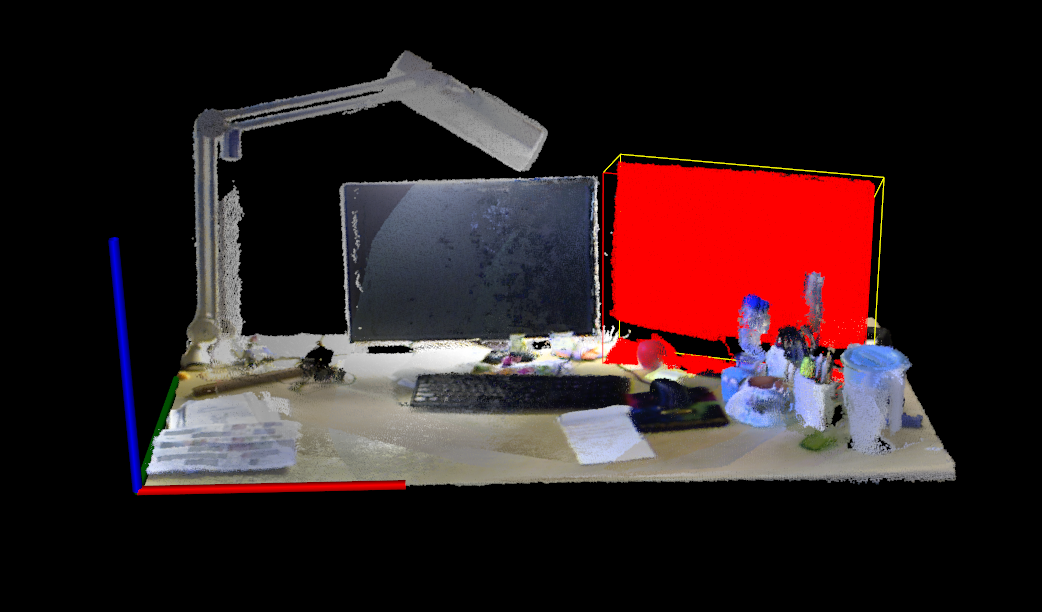
\includegraphics[scale = 0.30]{pcl_annotated.png}
\centering
\caption{\textbf{Annotated Point Cloud with Bounding Box over a Monitor \cite{KTH Dataset}}} 
\end{figure}

\subsection{Extraction of Features}

Using the information in the XML files obtained from the point cloud annotation tool, the following features shall be extracted \cite{STRANDS}, w.r.t a fixed frame of reference:

\paragraph{Single Object Features ($f_{o_i}$)}

\begin{itemize}
\item{3D position of the object centroid  (1 x 3)}
\item{2D (horizontal) bearing of object centroid, $\theta$ (1 x 1)}
\item{Volume of the object (1 x 1)}
\end{itemize}

\paragraph{Object Pair Features ($f_{o_i, o_j}$)}

\begin{itemize}
\item{$d(C_{o_i}$, $C_{o_j})$, where $d$ is the Euclidean distance and $C_{o_i}$, $C_{o_j}$ are the centroids of objects $o_i$ and $o_j$ respectively (1 x 1)}
\item{Ratio of the object volumes (1 x 1)}
\item{$d_z$($C_{o_i}$, $C_{o_j}$), where $d_z$ if the vertical displacement between the two objects (1 x 1)}
\end{itemize}

The possibility of adding more features which can improve the model shall also be explored in this thesis.


\begin{figure} [H]
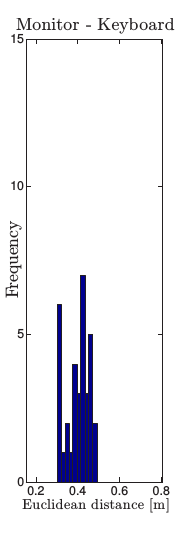
\includegraphics[scale = 0.50]{histogram.png}
\centering
\caption{\textbf{Histogram of one of the features, the Euclidean Distance between two objects \cite{KTH Dataset}}}
\end{figure}

In this way, each of the scenes from the set $S_t$, will be represented by a set of feature vectors. For example, if $s_1$ is a scene of a shelf with a book and a mug, then $s_1$ would be represented by $\{f_{book}, f_{mug}, f_{book, mug}\}$.  

\subsection{Fitting a Model}

Gaussian Mixture Models (GMMs) shall be used to model the aforementioned features.

\paragraph{Modeling Single Object Features:}

To model the single object features, we fit a GMM over each set of single object features collected from all the scenes:

\[
GMM(f_{o_i}, \mu_{o_i}^z, \Sigma_{o_i}^z) = \sum_{z=1}^{n_c} \pi_z \frac{1}{K}
exp(-\frac{1}{2} \zeta_{o_i}^z)
\]
where: 
\[\zeta_{o_i}^z = (f_{o_i} - \mu_{o_i}^z)^T \Sigma_{o_i}^{z - 1} (f_{o_i} - \mu_{o_i}^z)) \]
\[K = \sqrt{(2\pi)^{dim}|\Sigma_{o_i}^z|} \text{   ,   } 
\pi_z \geq 0 \text{   ,   }
\sum_{z = 1}^{d}\pi_z = 1\]
$n_c$ is the number of mixtures, $\pi_z$ is the weight of the $z^{th}$ mixture, $\mu_{o_i}^z$ is the mean of the normal distribution, $\Sigma_{o_i}^z$ is the covariance matrix and $dim$ is the dimensionality of the feature space.

Continuing on our example from earlier, we fit a GMM over all feature vectors of the object 'book' extracted from all scenes i.e. $GMM_{book}$ over $\{f_{book, s_{1}}, f_{book, s_{2}},...f_{book, s_{n}}\}$ and similarly, for other objects.

\paragraph{Learning object pair relationships:}

To learn these relationships, we fit a GMM again over each set of object pair features collected from all the scenes.

In other words, we fit $GMM_{book,mug}$ over $\{f_{book, mug, s_{1}}, f_{book, mug, s_{2}},....f_{book, mug, s_{n}}\}$ collected from all scenes.

Essentially, now we have condensed the scene type $S_t$ of that of a shelf to a set of GMMs: $\{GMM_{book}, GMM_{mug}, GMM_{book, mug}....\}$.


\subsection{Computation of Scene Similarity Score}

Now that we have modeled our scene with a set of GMMs, we present the program with a new unknown scene $s_u$ of a shelf with a few objects and the question becomes: how similar is this new unknown scene to our set of training scenes? Is there something off in this new scene?

For computing the scene similarity score, we extract the feature vectors from the new scene and use the fitted GMMs to compute the relative likelihood of these features belonging to the same distributions and hence, the same type of scene. 

Ideally, for implementation on a real robot, the feature extraction from the new scene should be performed automatically with the help of a perception software that is able to place 3D bounding boxes around objects, but that is outside the focus of this thesis, hence the new scene shall have a manually annotated point cloud as well.

Using the learned GMMs, the scene similarity score is predicted as a weighted sum as follows:

\[sim(s_u, S_t) = \sum_{o_i, o_j \in s_u} P(f_{o_i, o_j};S_t)P(o_i, o_j) + 
\sum_{o_i \in s_u} P(f_{o_i};S_t)P(o_i)\]
where $sim(s_u, S_t)$ is the scene similarity score of the new unknown scene $s_u$ with respect to the modeled scene class type $S_t$ and $f_{o_i}$, $f_{o_i, o_j}$ are feature vectors from the new scene. 

$P(f_{o_i, o_j};S_t)$ and $P(f_{o_i};S_t)$ are probability densities from the learned GMMs. $P(o_i, o_j)$ is computed from the frequency of co-occurence of objects $i$ and $j$ in all the scenes as:

\[P(o_i, o_j) = \frac{N_{o_i, o_j}}{N_{tot}}\]

where $N_{o_i, o_j}$ is the number of training scenes where both $o_i$ and $o_j$ are present and $N_{total}$ is the total number of training scenes. Similarly, $P(o_i)$ is computed from the frequency of occurence of object $o_i$ in all training scenes.

A threshold shall be fixed empirically after running the algorithm through some known anomalous scenes and this threshold shall then be used to detect future anomalous scenes. Furthermore, to identify the source of the anomaly in the scene, having thresholds for individual terms in the summation shall also be explored.






\section{Timeline}

\begin{figure} [H]
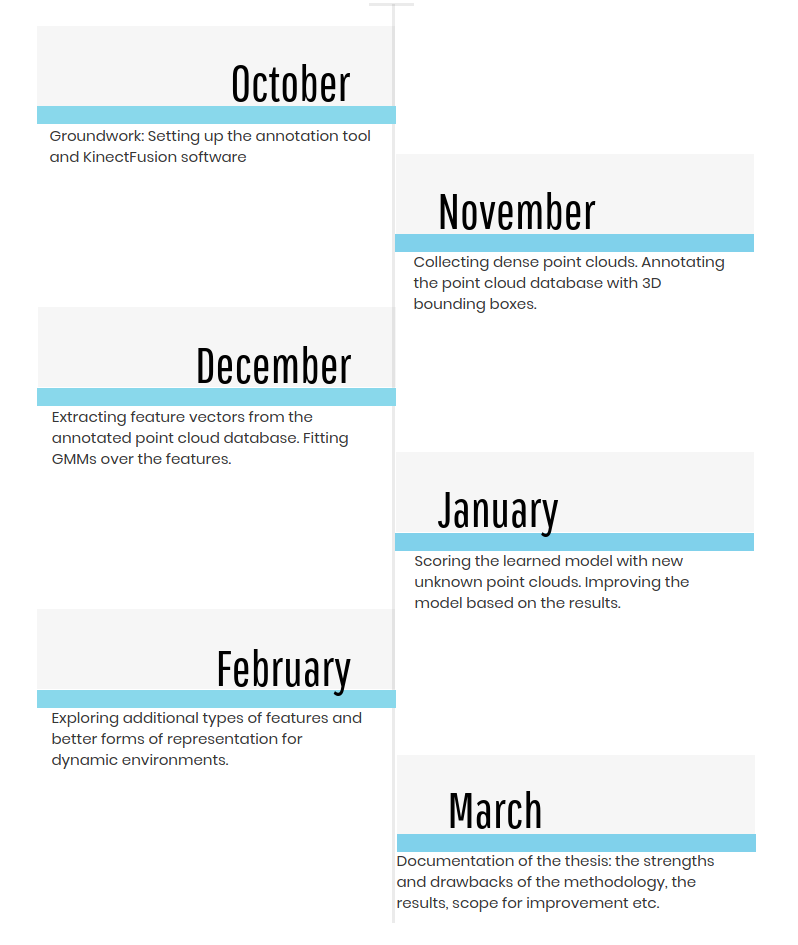
\includegraphics[scale = 0.60]{timeline3.png}
\centering

\end{figure}

%\newpage
%
%\section{References}
%
%\begin{enumerate}
%\item{M. Alberti, J. Folkesson and P. Jensfelt. Relational Approaches for Joint Object Classification and Scene Similarity Measurement in Indoor Environments. \textit{AAAI Spring Symposium,} 2014}
%\item{R. Newcombe, et al. KinectFusion: Real-Time Dense Surface Mapping and Tracking. \textit{ISMAR,} 2011}
%\end{enumerate}


\newpage

\begin{thebibliography}{9}

\bibitem{STRANDS} 
M. Alberti, J. Folkesson and P. Jensfelt. 
\textit{Relational Approaches for Joint Object Classification and Scene Similarity Measurement in Indoor Environments}. 
AAAI Spring Symposium, 2014.
 
\bibitem{KinectFusion} 
R. Newcombe, et al. 
\textit{KinectFusion: Real-Time Dense Surface Mapping and Tracking}. 
ISMAR, 2011.

\bibitem{KTH Dataset} 
A. Thippur, et al. 
\textit{KTH-3D-TOTAL: A 3D Datset for Discovering Spatial Structures for Long-Term Autonomous Learning}. 
ICARCV, 2014.
 
\end{thebibliography}

\end{document}










